\section{Сглаживание биржевых данных}

\subsection{Постановка задачи}
В рамках данного раздела рассматривается задача сглаживания реальных биржевых данных (котировок акций ПАО «Сбербанк» за период 2022–2026 гг.) с помощью линейного динамического фильтра нижних частот первого порядка.

Входным сигналом $u(t)$ является ежедневная цена закрытия акций. Динамика фильтра первого порядка описывается дифференциальным уравнением:
\begin{equation}
    T \frac{dy(t)}{dt} + y(t) = u(t)
\end{equation}
где $T$ — постоянная времени фильтра, определяющая его инерционность и частоту среза $\omega_c = 1/T$, а $y(t)$ — сглаженный выходной сигнал.

Передаточная функция непрерывного фильтра имеет вид:
\begin{equation}
    W(p) = \frac{1}{Tp + 1}
\end{equation}

Моделирование процесса фильтрации во временной области реализуется численно с использованием функции \texttt{lsim}. Согласно заданию, исследование проводится для пяти различных значений постоянной времени $T$: 1 день, 1 неделя, 1 месяц, 3 месяца и 1 год.

\paragraph{Учет ненулевых начальных условий}

Стандартная реализация функции линейного моделирования \texttt{lsim} по умолчанию предполагает, что в начальный момент времени ($t = 0$) система находится в состоянии покоя, то есть вектор начальных состояний равен нулю.

Однако для биржевых котировок такое допущение некорректно, в первый день выборки базовая цена акции отлична от нуля. Если не учесть этот факт, фильтр будет совершать резкий скачок из нуля, порождая длительный искусственный переходный процесс.

Для устранения данного дефекта в алгоритм численного расчета были принудительно заложены ненулевые начальные условия. Начальное состояние фильтра первого порядка было принято равным первому известному значению котировок акций

\begin{equation}
    X_0 = [u[0]]
\end{equation}

Это позволило совместить точку старта фильтрованного сигнала с реальным началом
временного ряда и полностью ликвидировать паразитный переходный процесс.

\subsection{Результаты моделирования}

Ниже представлены сравнительные графики исходного курса акций и результатов линейной фильтрации для каждого из заданных значений постоянной времени $T$. На каждом рисунке совмещены два масштаба отображения: временной диапазон порядка $T$ (для детального анализа фазового сдвига) и весь доступный массив данных за несколько лет.

\begin{figure}[H]
    \centering
    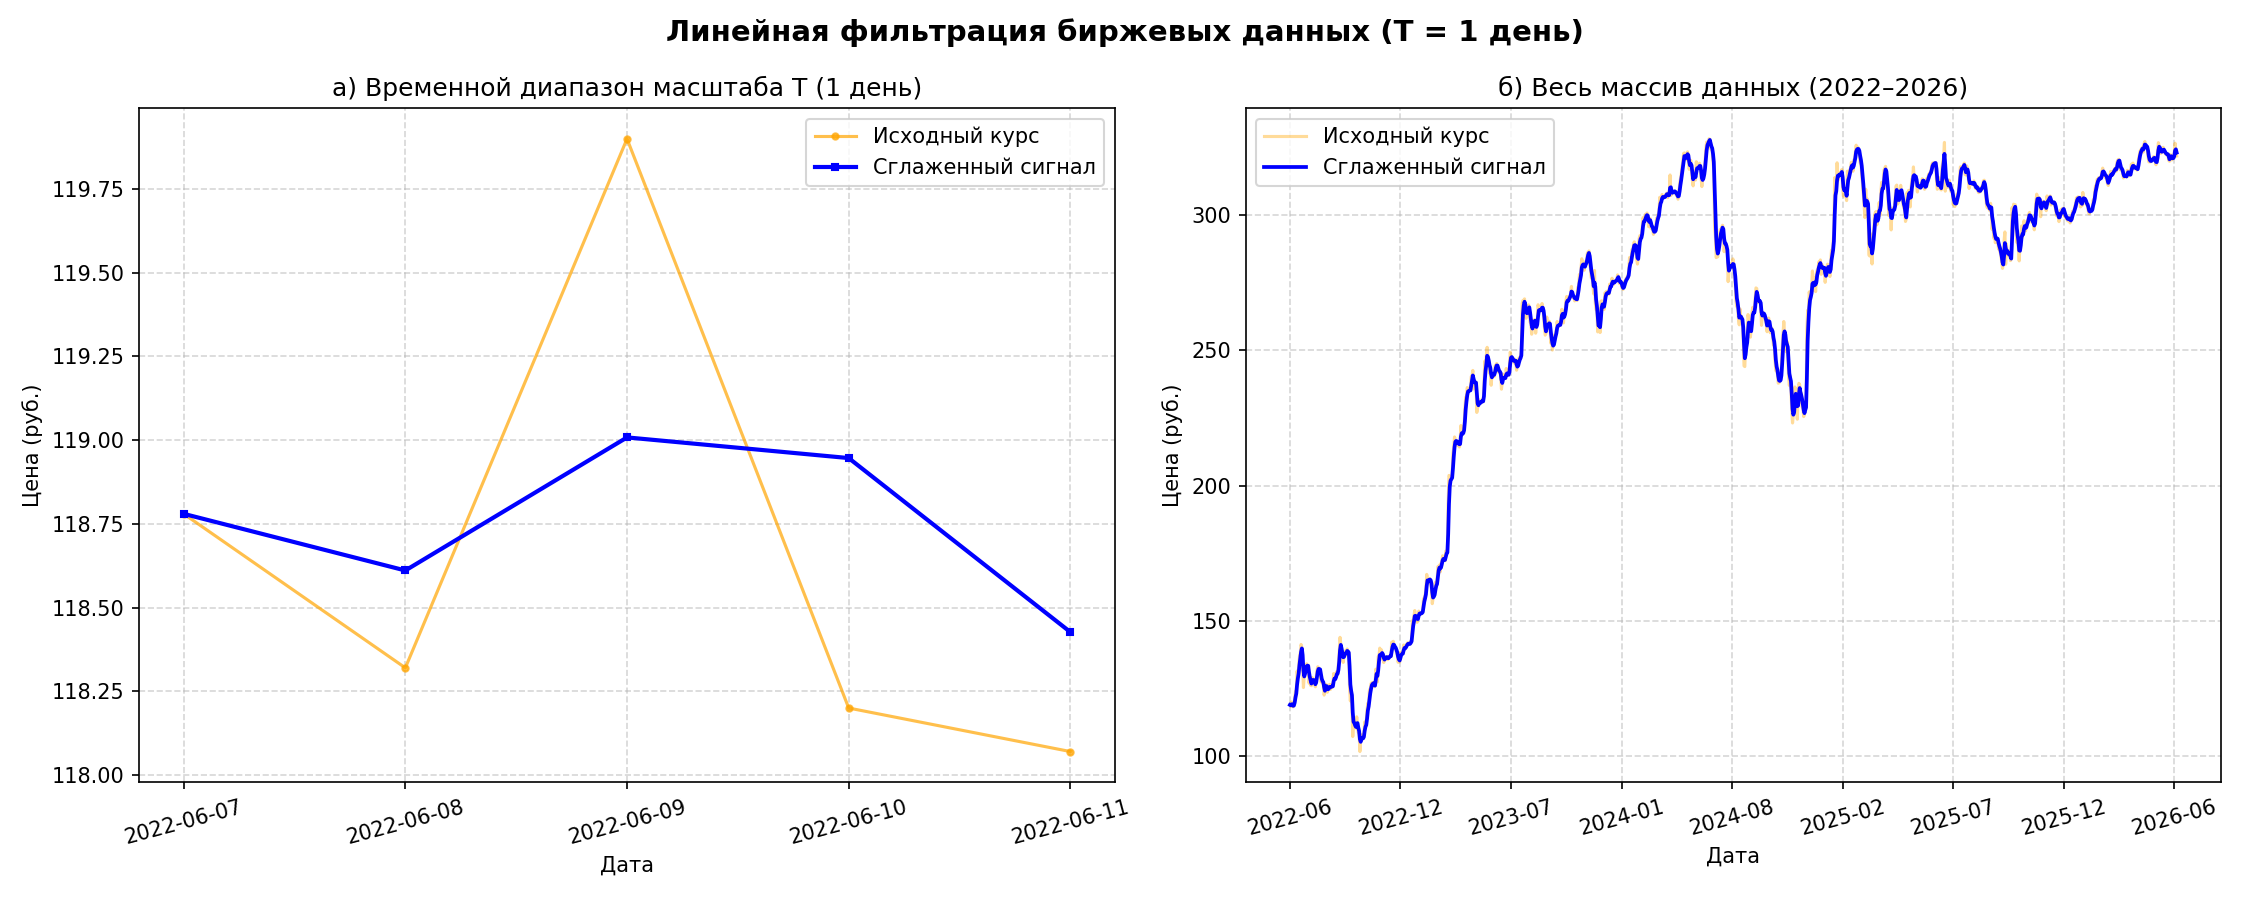
\includegraphics[width=\textwidth]{images/3_3/task_3_3_1_day.png}

\end{figure}

\begin{figure}[H]
    \centering
    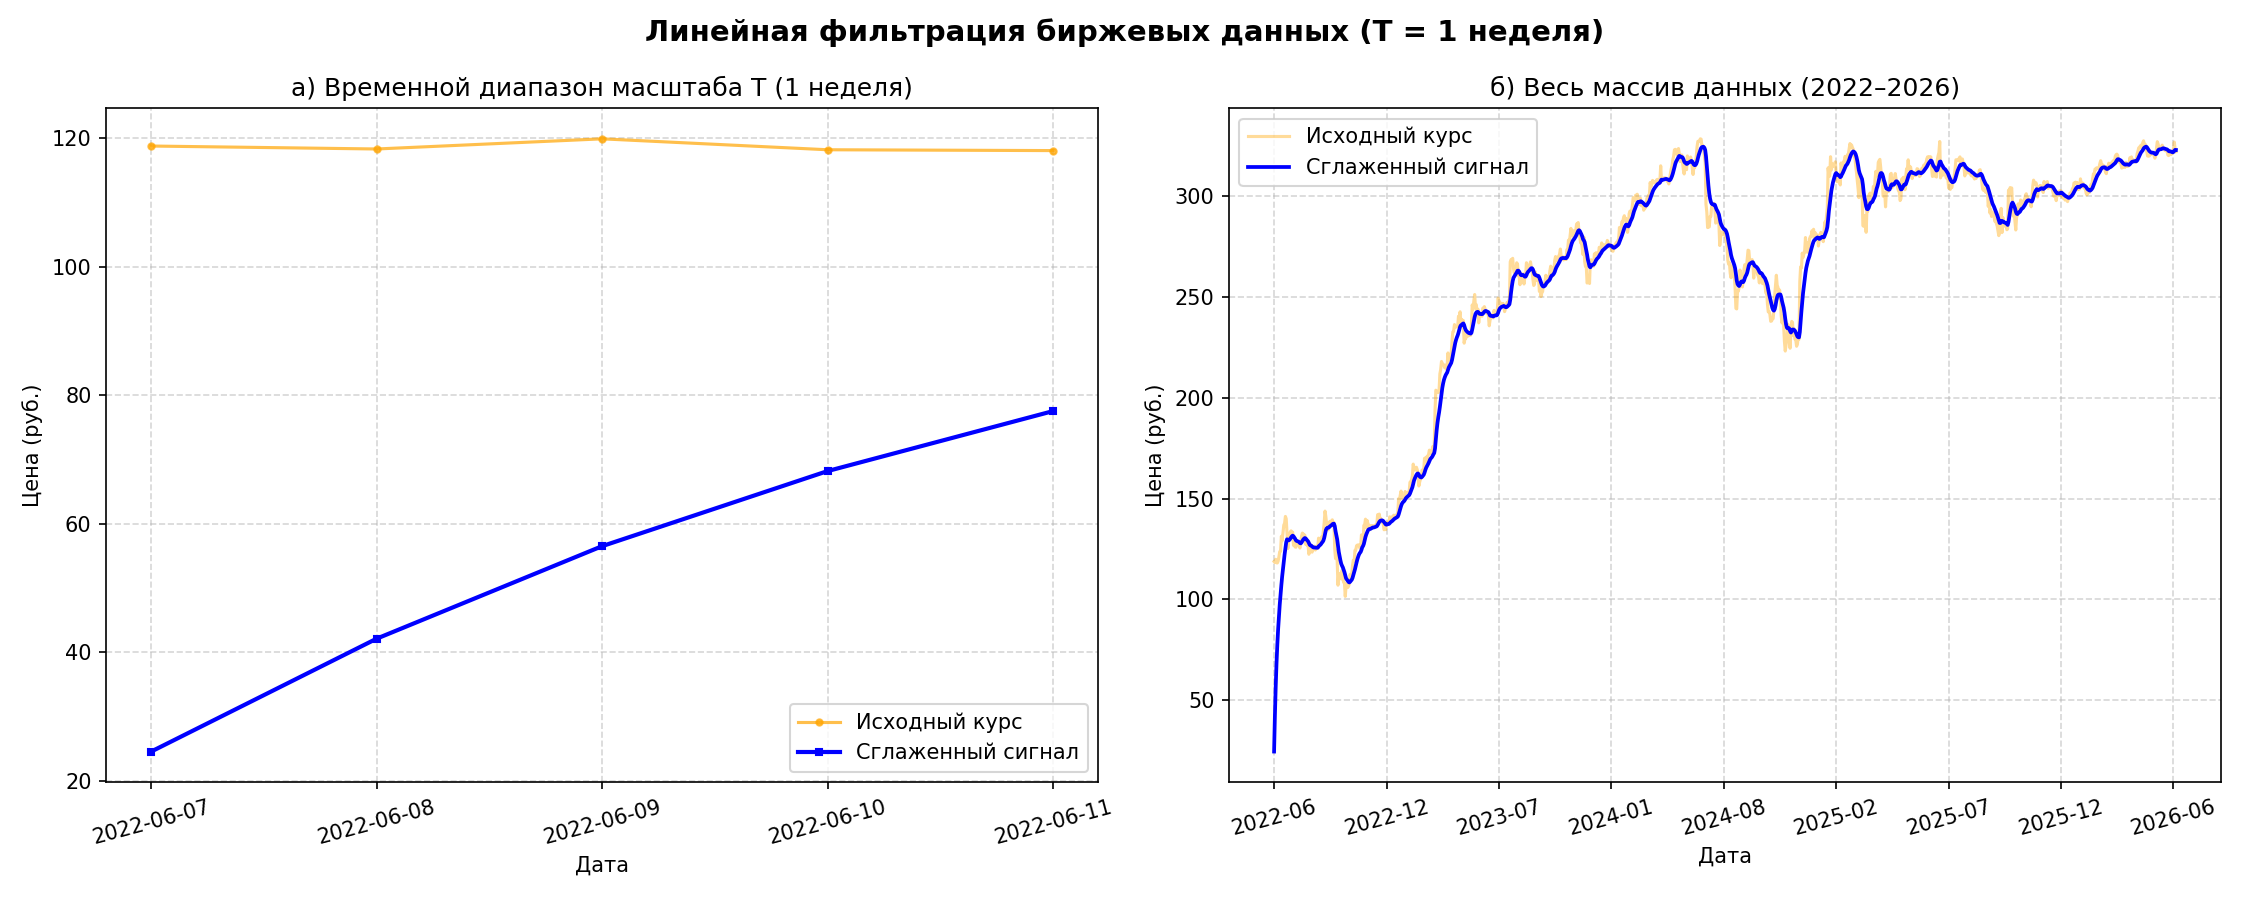
\includegraphics[width=\textwidth]{images/3_3/task_3_3_1_week.png}

\end{figure}

\begin{figure}[H]
    \centering
    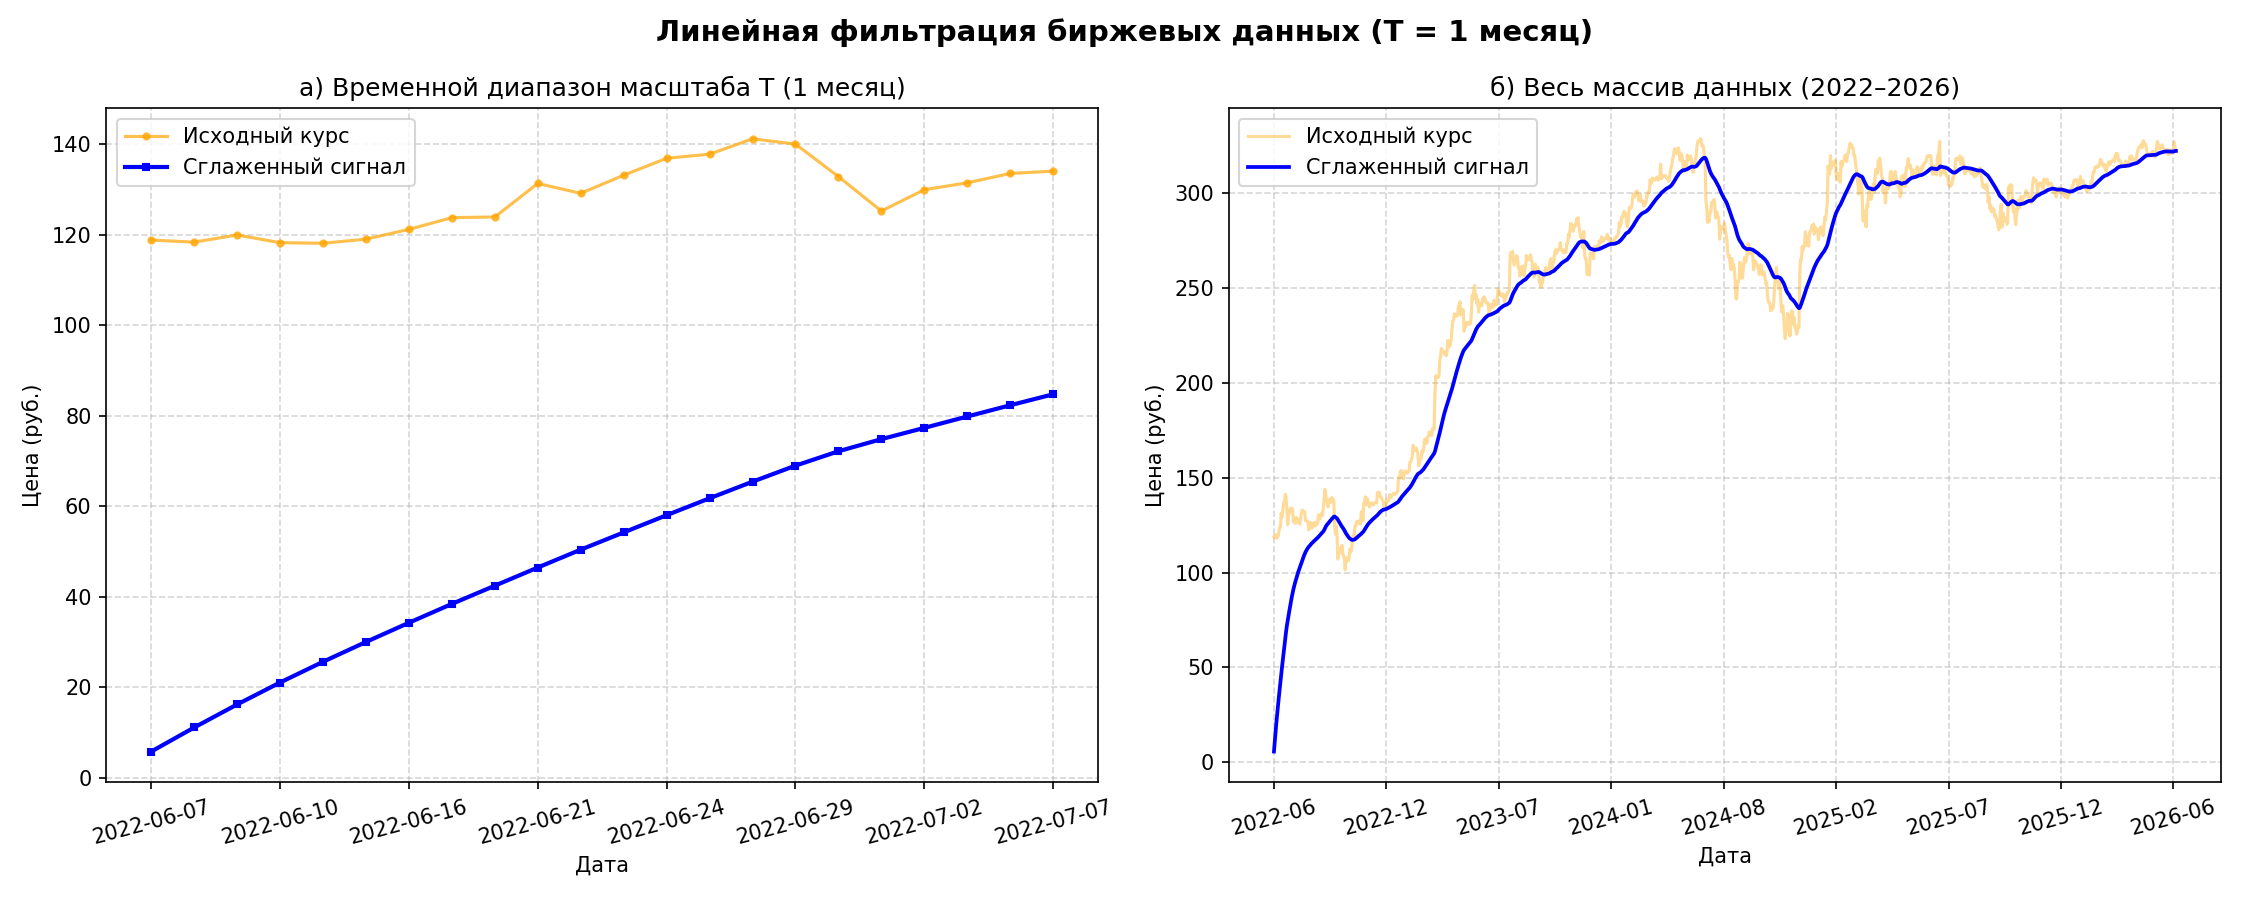
\includegraphics[width=\textwidth]{images/3_3/task_3_3_1_month.png}

\end{figure}

\begin{figure}[H]
    \centering
    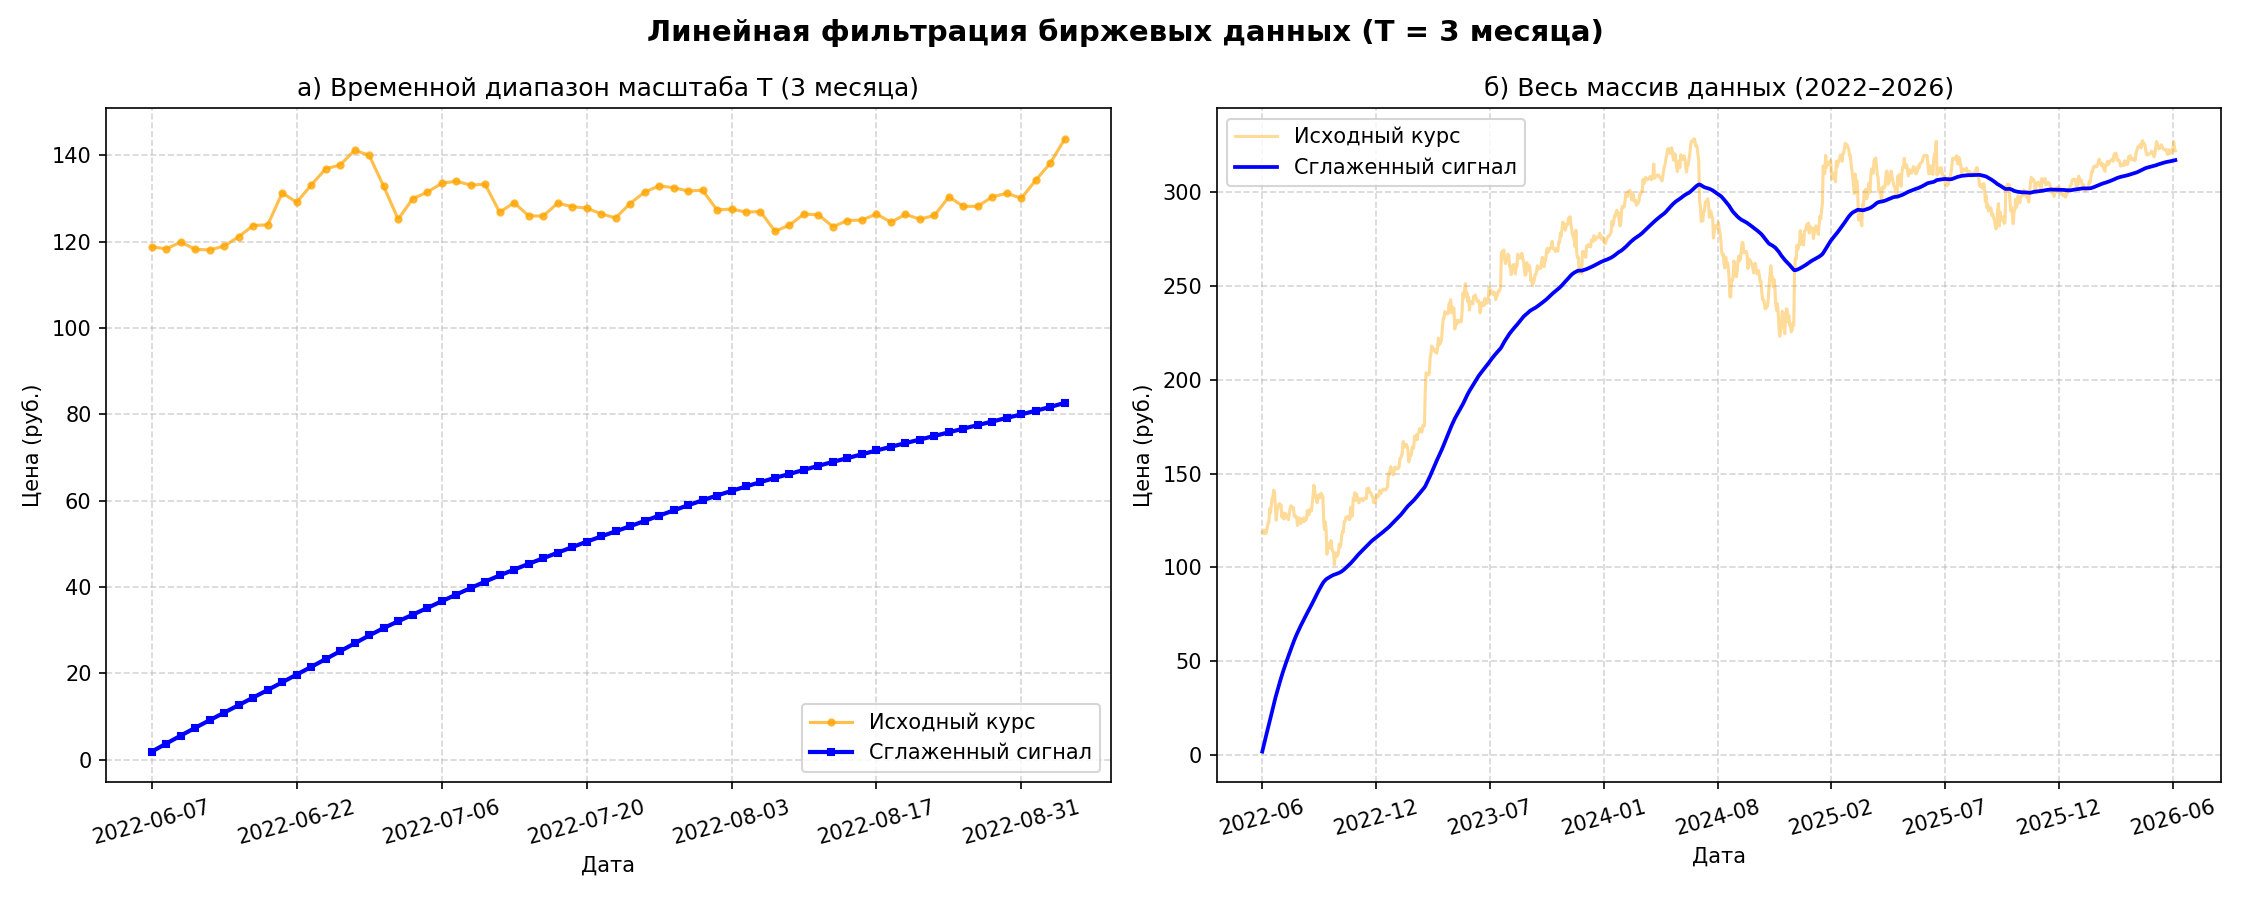
\includegraphics[width=\textwidth]{images/3_3/task_3_3_3_months.png}

\end{figure}

\begin{figure}[H]
    \centering
    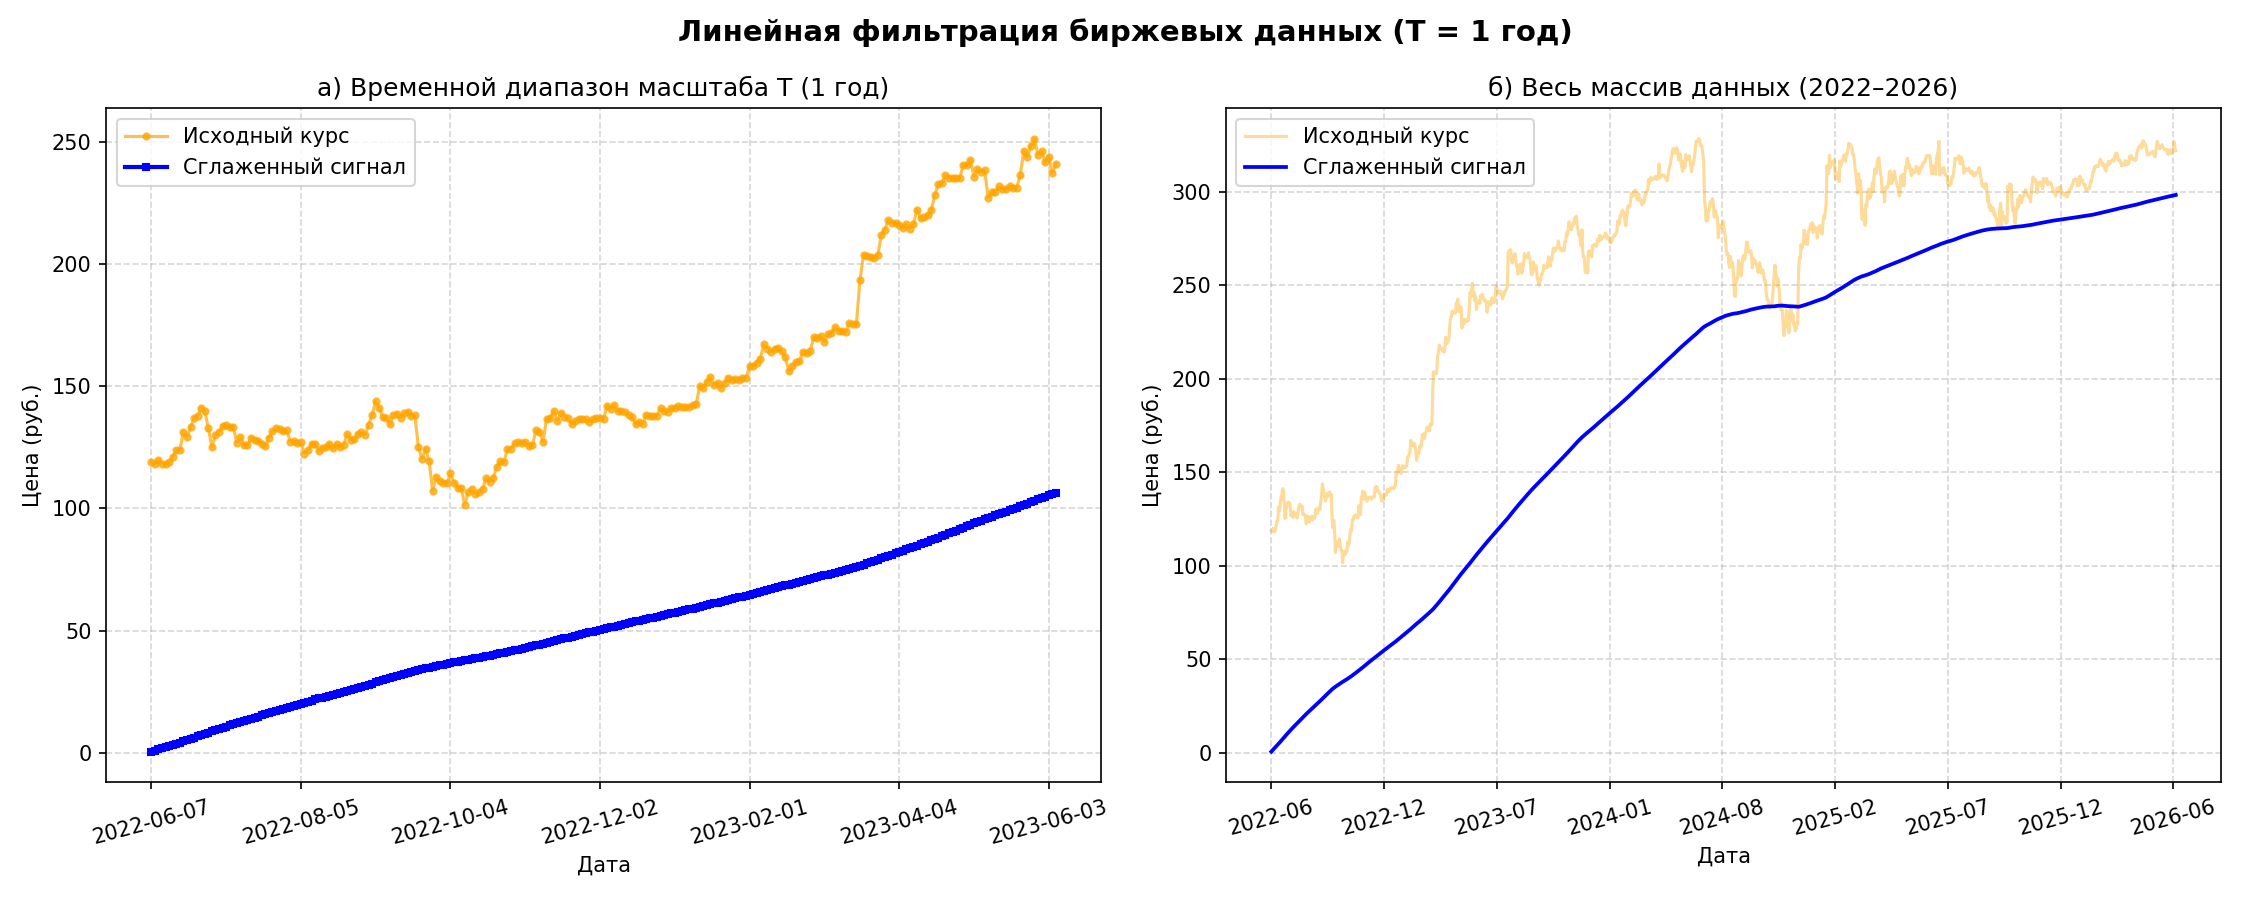
\includegraphics[width=\textwidth]{images/3_3/task_3_3_1_year.png}

\end{figure}

\subsection{Анализ результатов и выводы}

На основе полученных графических зависимостей можно провести детальный анализ влияния постоянной времени $T$ на качество динамической фильтрации:

\begin{itemize}
    \item \textbf{малые значения $T$ ($1$ день, $1$ неделя):} Фильтр обладает высокой частотой среза и минимальной инерционностью. Сглаженная кривая практически мгновенно реагирует на любые локальные изменения тренда, фазовая задержка визуально незаметна. Однако качество подавления высокочастотного шума (дневной волатильности рынка) остается низким — отфильтрованный сигнал сохраняет сильную изрезанность.

    \item \textbf{средние значения $T$ ($1$ месяц, $3$ месяца):} Достигается оптимальный баланс. Фильтр успешно подавляет краткосрочные спекулятивные колебания («шум» рынка) и локальные ценовые выбросы, выделяя устойчивые среднесрочные тренды. При этом возникающий фазовый сдвиг (запоздание сигналов покупки/продажи относительно экстремумов реальной цены) остается в допустимых пределах.

    \item \textbf{большое значение $T$ ($1$ год):} Фильтр становится крайне тяжелым и инерционным. Частота среза смещается глубоко в низкочастотную область. На выходе формируется идеально гладкая линия, отражающая исключительно глобальный долгосрочный (многолетний) тренд стоимости компании. Обратной стороной такой глубокой фильтрации становится колоссальное фазовое запаздывание — реакция на разворот рынка отстает на месяцы, что делает такой фильтр неприменимым для оперативного трейдинга, но полезным для макроэкономического анализа.
\end{itemize}

\paragraph{Выводы}
В ходе выполнения задания была эмпирически подтверждена фундаментальная закономерность динамической фильтрации: выбор параметров фильтра всегда представляет собой компромисс между качеством подавления нежелательных высокочастотных изменений и величиной фазового запаздывания полезного сигнала.

Кроме того, была доказана критическая важность корректного задания начальных условий в задачах численного моделирования реальных процессов. Введение ненулевого начального условия вида $X_0 = [u[0]]$ позволило полностью исключить переходные процессы, обеспечив корректность работы ФНЧ с первого шага временной сетки.